\begin{figure}[h]
\textbf{Tema d'Esame di Gennaio 2018}\\ \\
Una massa $M = 100 g$ viene lanciata con un sistema come quello in figura. Se la costante elastica della molla è $k = 500 N/m$, quale deve
essere la sua compressione perché la massa $M$ raggiunga un’altezza massima
$h = 2.00 m$ da terra. Il tratto inclinato forma un angolo $\theta$ = 20.0$^{\circ}$ con il terreno, è lungo $L = 50.0 cm$ e ha un coefficiente di attrito $f = 0.10$
\\
	\begin{center}
		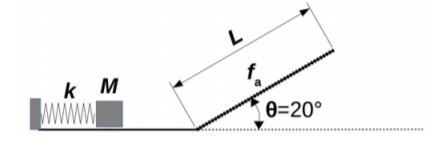
\includegraphics[scale=0.8]{ES2/GEN022018.jpg}
	\end{center}
\end{figure}